% time values for run2/10, run4/11, run15/16
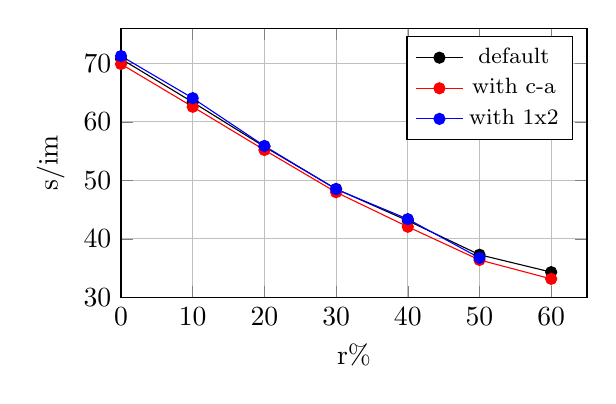
\begin{tikzpicture}
\begin{axis}[
    title={},
    height=5cm,
    width=7.5cm,
    xlabel={r\%},
    ylabel={s/im},
    xmin=0, xmax=65,
    ymin=30, ymax=76,
    xtick={0,10,20,30,40,50,60},
    ytick={30,40,50,60,70},
    legend pos=north east,
    xmajorgrids=true,
    ymajorgrids=true,
    legend style={font=\footnotesize}
]

\addplot[
    color=black,
    mark=*
    ]
    coordinates {
    (0,70.76)(10,63.36)(20,55.75)(30,48.53)(40,43.10)(50,37.29)(60,34.32)
    };
    
\addplot[
    color=red,
    mark=*
    ]
    coordinates {
    (0,69.88)(10,62.57)(20,55.19)(30,47.97)(40,42.07)(50,36.40)(60,33.16)
    };

\addplot[
    color=blue,
    mark=*
    ]
    coordinates {
    (0,71.25)(10,64.05)(20,55.88)(30,48.49)(40,43.38)(50,36.75)
    };
    
\legend{default, with c-a, with 1x2}
    
\end{axis}
\end{tikzpicture}